\documentclass[letterpaper, 12pt]{article}
\usepackage[top=.5in,bottom=.5in,left=.75in,right=.75in,headheight=30pt, % as per the warning by fancyhdr
includehead,includefoot,
heightrounded, % to avoid spurious underfull messages
]{geometry}
\addtolength{\topmargin}{-.25in}
\usepackage{fancyhdr}
\pagestyle{fancy}
\usepackage{graphicx}
\usepackage{lastpage}
\usepackage{multicol}
\usepackage{qrcode}
\usepackage{gensymb}
\usepackage{pgfplots}

\begin{document}
\fancyhead[l]{	\includegraphics[height=0.5in]{../Logo/sp.png} Name:}
\fancyhead[r]{Due Date: \hspace{ 1in}}
\fancyfoot[c]{\thepage\ of \pageref{LastPage}}
\fancyfoot[r]{Assignment 3.01}	


\begin{center} Assignment 3.02: Velocity vs Time Graphs

\vspace{0.1in}
	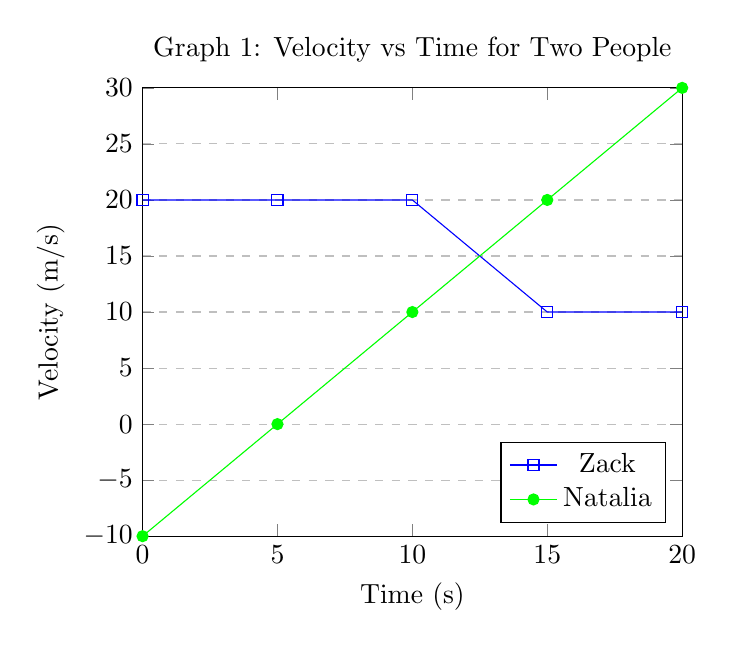
\begin{tikzpicture}
\begin{axis}[
title={Graph 1: Velocity vs Time for Two People},
xlabel={Time (s)},
ylabel={Velocity (m/s)},
xmin=0, xmax=20,
ymin=-10, ymax=30,
xtick={0,5,10,15,20},
ytick={-10,-5,0,5,10,15,20,25,30},
ymajorgrids=true,
grid style=dashed,
legend pos=south east,
]

\addplot[
color=blue,
mark=square,
]
coordinates {
	(0,20)(5,20)(10,20)(15,10)(20,10)};
\addlegendentry{Zack}

\addplot[
color=green,
mark=*,
]
coordinates {
	(0,-10)(5,0)(10,10)(15,20)(20,30)};
\addlegendentry{Natalia}



\end{axis}
\end{tikzpicture}
\end{center}


\begin{enumerate}
 \item  \vspace{-.2in} Use Graph 1 to determine the following: \vspace{-.1in}
\begin{enumerate}
	\item Who is moving faster at t=5 seconds? \vspace{.25in}
	\item How far has Natalia traveled by t=10 seconds?  \vspace{.25in}
	\item What is Zack's acceleration?\vspace{.25in}
	\item What is Natalia's acceleration?\vspace{.25in}
	\item Assuming both people start in the same place, who travels farther?  Explain your reasoning.\vspace{.25in}
	\item Graph 1 describes a race between Zack and Natalia.  In at least 4 complete sentences, describe what happened during this race. \vspace{1in}
\end{enumerate}


\pagebreak

	\item Use the graphs to answer the following questions:
	
	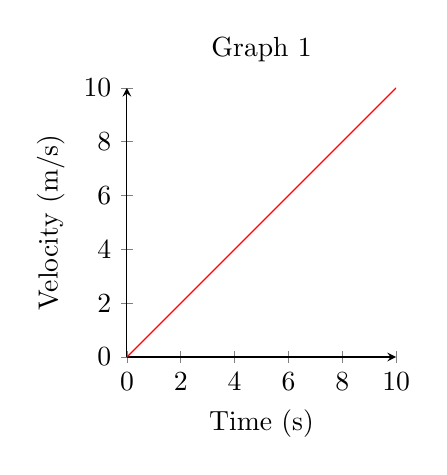
\begin{tikzpicture}
	\begin{axis}[title=Graph 1, xlabel=Time (s), ylabel=Velocity (m/s), axis lines = left, width=5cm,height=5cm]
	% density of Normal distribution:
	\addplot
	[
	red,
	domain
	=0:10,
	samples
	=201,
	]
	{x};
	\end{axis}
	\end{tikzpicture}%
	%
	%
	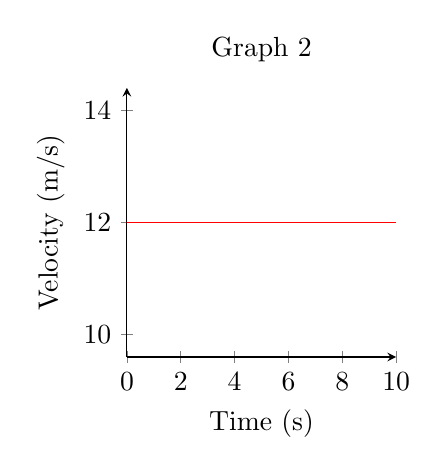
\begin{tikzpicture}
	\begin{axis}[title=Graph 2, xlabel=Time (s), ylabel=Velocity (m/s), axis lines = left, width=5cm,height=5cm]
	% density of Normal distribution:
	\addplot
	[
	red,
	domain
	=0:10,
	samples
	=201,
	]
	{12};
	\end{axis}
	\end{tikzpicture}%	
	%
	%
	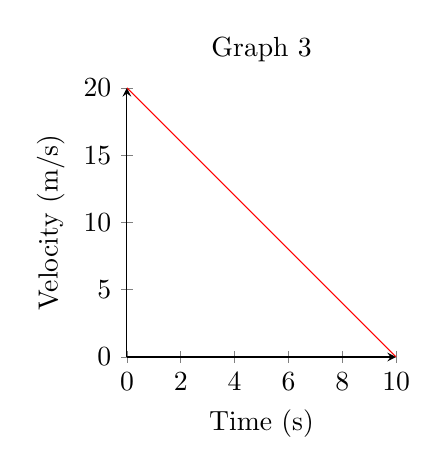
\begin{tikzpicture}[]
	\begin{axis}[title=Graph 3, xlabel=Time (s), ylabel=Velocity (m/s), axis lines = left, width=5cm,height=5cm]
	% density of Normal distribution:
	\addplot
	[
	red,
	domain
	=0:10,
	samples
	=201,
	]
	{-2*x+20};
	\end{axis}
	\end{tikzpicture}%


\begin{enumerate}
	\item Graph 1: 
	\begin{enumerate}
		\item Describe the motion of the object in one sentence.
		\vspace{0.3in}
		\item Determine the acceleration of the object.
		\vspace{0.3in}
		\item Determine the distance traveled in 10 seconds.
		\vspace{0.3in}
		
	\end{enumerate}
	\item Graph 2:
		\begin{enumerate}
		\item Describe the motion of the object in one sentence.
		\vspace{0.3in}
		\item Determine the acceleration of the object.
		\vspace{0.3in}
		\item Determine the distance traveled in 10 seconds.
		\vspace{0.3in}
		
	\end{enumerate}

	\item Graph 3:
		\begin{enumerate}
		\item Describe the motion of the object in one sentence.
		\vspace{0.3in}
		\item Determine the acceleration of the object.
		\vspace{0.3in}
		\item Determine the distance traveled in 10 seconds.
		\vspace{0.3in}
		
	\end{enumerate}
	
	
	
	\end{enumerate}

\newpage
\item Sketch a graph that corresponds to each situation below:
\begin{enumerate}
	\item A car is parked.
	\item A truck drives forward 10 meters at a constant speed, then stops.
	\item A lion runs forward, then stops, then walks back to where it started.
\end{enumerate}

	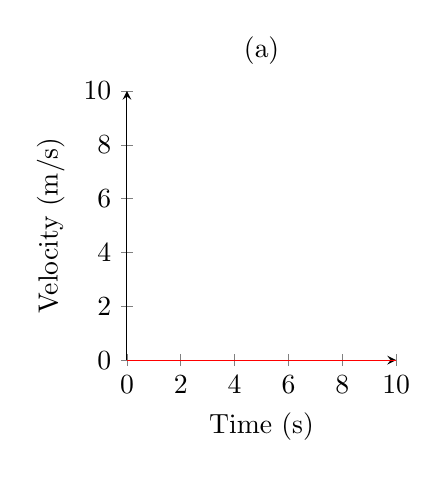
\begin{tikzpicture}
\begin{axis}[title=(a), xlabel=Time (s), ylabel=Velocity (m/s), width=5cm,height=5cm,  ymin=0, ymax=10,axis lines=left]
% density of Normal distribution:
\addplot
[
red,
domain
=0:10,
samples
=201,
]
{0};
\end{axis}
\end{tikzpicture}%
%
%
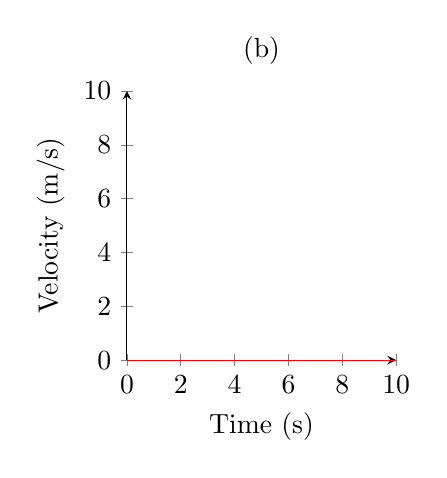
\begin{tikzpicture}
\begin{axis}[title=(b), xlabel=Time (s), ylabel=Velocity (m/s), axis lines = left, width=5cm,height=5cm, ymin=0, ymax=10]
% density of Normal distribution:
\addplot
[
red,
domain
=0:10,
range=0:10,
samples
=201,
]
{0};
\end{axis}
\end{tikzpicture}%	
%
%
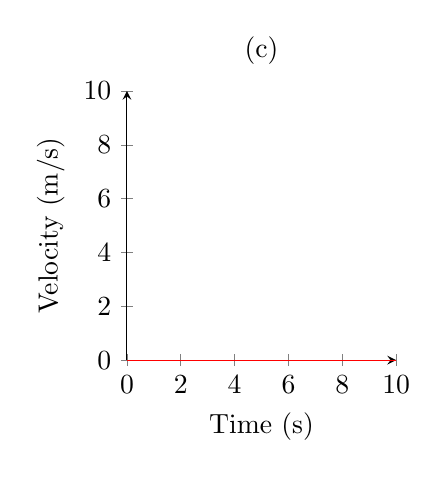
\begin{tikzpicture}[]
\begin{axis}[title=(c), xlabel=Time (s), ylabel=Velocity (m/s), axis lines = left, width=5cm,height=5cm, ymin=0, ymax=10]
% density of Normal distribution:
\addplot
[
red,
domain
=0:10,
samples
=201,
]
{0};
\end{axis}
\end{tikzpicture}%


\end{enumerate}
\end{document}
